\chapter{Grundlagen}

%%%%%%%%%%%%%%%%%%%%%%%%%%%%%%%%%%%%%%%%%%%%%%%%%%%%%%%%%%%%%%%%%%%%%%%%%%%%%%%%%%%%%%%%%%%%%%%%%%%%%%%%%%%%%%%
%
%						DOMAIN	DRIVEN	DESIGN
%
%%%%%%%%%%%%%%%%%%%%%%%%%%%%%%%%%%%%%%%%%%%%%%%%%%%%%%%%%%%%%%%%%%%%%%%%%%%%%%%%%%%%%%%%%%%%%%%%%%%%%%%%%%%%%%%

\section{Domain-Driven Design}

\subsection{Definition}

Die Domäne einer Software bezeichnet das Themengebiet oder den Anwendungsbereich, in dem das Programm eingesetzt wird \cite[S.2]{evans} \cite[S.307]{posch}. \glqq Domain-Driven Design\grqq{} (Abk.: DDD) ist eine Herangehensweise, Problemdomänen in ein Modell für die Softwareentwicklung zu überführen. Modellieren ist eine grundlegende Methode der Wissenschaft um mit komplexen Systemen umzugehen. Eine Abstraktion eines solchen Systems, die es ermöglicht, Fragestellungen dazu zu beantworten, wird als Modell bezeichnet \cite{brugge}.

Geprägt wurde das DDD durch Eric Evans in seinem Buch \glqq Domain-Driven Design: Tackling Complexity in the Heart of Software\grqq{} \cite{evans}. Kern des domänengetriebenen Entwurfs ist es, die reale, oft unübersichtliche Fachlichkeit fortschreitend in feiner geschnittene Teilbereiche zu kapseln. Diese sollen möglichst wenige Abhängigkeiten zueinander haben \cite[S.63, 70]{dowalil}. Dieser auf das Domänenmodell fokussierte Ansatz versucht, Kernaspekte einer Anwendung in das Modell zu integrieren, anstatt sie über externe Dienste einzubinden \cite[S.74]{daschner}.

Evans stellt drei Grundeigenschaften fest, welche bei der Wahl eines Modells im DDD zu berücksichtigen sind \cite[S. 3-4]{evans}:
\begin{itemize}
\item Es existiert immer eine Abhängigkeit zwischen Modell und Implementierung.
\item Die Terminologie während der Softwareentwicklung ist eine Implikation des zugrunde liegenden Modells.
\item Nützliches und aufgearbeitetes Wissen kann diesem Modell entnommen werden.
\end{itemize}

Ein weiteres Kernkonzept des DDD ist die \glqq Ubiquitous Language\grqq{}. Sie verbindet Entwickler und Domänen-Experten durch eine auf dem Modell basierende Sprache. Dabei definiert sie eindeutig die verwendeten Begriffe und die ihnen zugeordneten Fachlichkeiten \cite[S. 25-27]{evans}. Ein weiterer Kern ist das \glqq Model-Driven Design\grqq{{} (Abk.: MDD). MDD betont und bezeichnet das notwendige Ineinandergreifen der Konzeption eines Domänenmodells mit dem Entwurf der Anwendungssoftware. Um eine enge Übereinstimmung zwischen Modell und Software sicherzustellen, ist es von Vorteil, innerhalb eines durch Software-Tools unterstützten Modellierungsansatzes zu arbeiten. Objektorientierte Programmiersprachen eignen sich besonders gut, da sich die objekthaften Eigenschaften von Modellen gut abbilden lassen \cite[S. 49-51]{evans}.


\pagebreak 
\subsection{Bausteine des Model-Driven Design}

Das DDD definiert verschiedene Bausteine des MDD \cite[S. 65]{evans}:

\begin{figure}[ht]
\centering
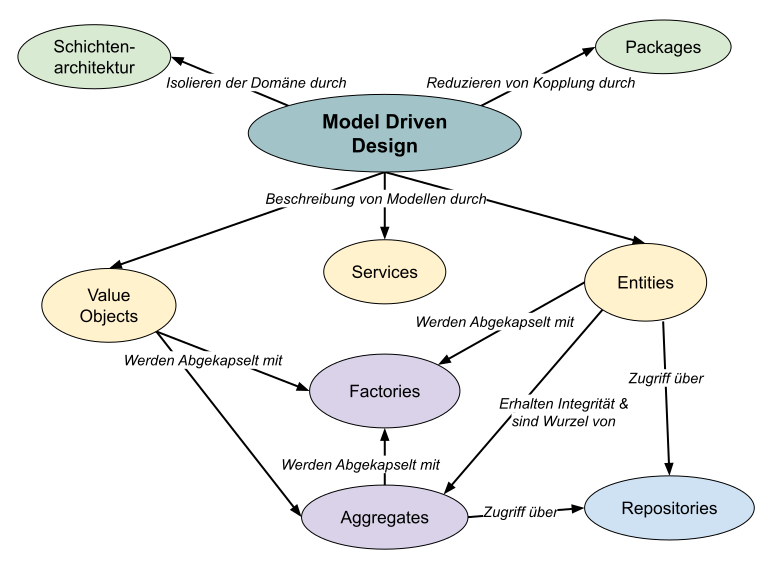
\includegraphics[width=\textwidth]{bilder/k2/MDD.pdf}
\caption[Bausteine des Model-Driven Design]{Die Bausteine des Model-Driven Design und wie Sie im Kontext zu anderen Bausteinen einzuordnen sind}
\end{figure}

\subsubsection{Schichtenarchitektur}


Der schichtbasierte Architekturstil teilt Software in verschiedene Schichten auf. Jede Schicht fasst Komponenten zusammen, die ähnliche Aufgaben haben. Das macht die Software einfacher zu verstehen und zu verwalten. Die Architektur ist nach technischen Funktionen gegliedert. Gängige Schichten sind die Präsentationsschicht, Geschäftslogikschicht, Persistenzschicht, Datenbankschicht oder die Dienstschicht. Jedes Element einer Schicht hängt nur von Elementen derselben oder einer tieferen Schicht ab. DDD fordert, die Geschäftslogik in eine eigene Schicht, der \glqq Domain Layer\grqq, zu legen. Dies sorgt für eine enge Verbindung zum Modell, wie es das MDD vorsieht \cite[S. 69 - 73]{evans} \cite[S.139-141]{richards}.


\subsubsection{Packages}

\glqq Packages\grqq, auch als \glqq Modules\grqq{} bezeichnet, sorgen im Modell für starke Kohäsion innerhalb und schwache Kopplung zwischen ihnen, indem sie zusammengehörige Elemente bündeln \cite[S. 109 - 116]{evans}.

\subsubsection{Entities}

\glqq Entities\grqq{} sind einzigartige, identifizierbare Objekte eines speziellen Bereichs. Dies kann z.B. mit automatisch erzeugten Identifikationswerten (Abk.: ID) umgesetzt werden. Ihre spezifischen Merkmale sind sekundär. Sie symbolisieren die durchgehende Existenz eines Objekts über dessen Lebenszyklus. Beim Erstellen eines Modells muss diese Kontinuität gewährleistet werden. Klassendetails, Aufgaben und Assoziationen sollten ebenso die Identität der Entity zeigen. Entities sollen sparsam verwendet werden. Nur notwendiges Verhalten soll ihnen hinzugefügt werden. Zusätzliches Verhalten soll zu anderen zugehörigen Objekten verschoben werden \cite[S. 89-96]{evans} \cite[S.75]{daschner}.

\subsubsection{Value Objects}

\glqq Value Objects\grqq{} sind Typen ohne eigene Identität, die spezifische Werte repräsentieren. Sie können aus anderen Value Objects bestehen und Entities referenzieren. Oft werden sie als Parameter zwischen Objekten oder als Eigenschaften von Entities genutzt. Value Objects sollten eine hohe Kohäsion besitzen und sind unveränderlich, um sicher geteilt werden zu können. Bidirektionale Verbindungen bei Value Objects sollten aufgrund ihrer fehlenden Identität vermieden werden \cite[S. 97-103]{evans} \cite[S.75]{daschner}.

\subsubsection{Services}

\glqq Services\grqq{} bieten eine spezielle Funktion im Modell an, ohne dabei Daten oder Zustände zu speichern. Sie werden dabei nach ihrer Aufgabe benannt. Services starten Vorgänge und arbeiten mit den Objekten des Modells. Sie kombinieren Schritte in Geschäftsprozessen und sollten bedacht eingesetzt werden. Außerdem sollen sie nicht alle Aufgaben von Entities und Value Objects abnehmen. Es existiert eine klare Schnittstelle im Bezug auf andere Elemente des Modells. Da Services auch außerhalb der Domain Layer auftreten können ist eine präzise fachliche Betrachtung nötig \cite[S. 104 - 108]{evans} \cite[S.74]{daschner}.

\subsubsection{Aggregates}

\glqq Aggregates\grqq{} sind Ansammlungen von Objekten, die zusammen als Einheit betrachtet werden. Ihr Zweck ist es, Veränderungen als Ganzes zu handhaben, um Konsistenz zu gewährleisten. Ein direkter Zugriff auf einzelne Bestandteile ist nicht möglich. Deswegen gibt es in einem Aggregate ein Hauptobjekt (Wurzel), das für alle Aktionen verwendet wird. Andere Objekte können nur auf dieses Hauptobjekt verweisen, wobei die enthaltenen Objekte sich untereinander gegenseitig verweisen können. Objekte innerhalb des Aggregates, die nicht die Hauptfunktion ausüben, sind nur in ihrem Kontext eindeutig identifizierbar \cite[S. 123 - 135]{evans} \cite[S.76]{daschner}.

\subsubsection{Factories}

Eine \glqq Factory\grqq{} erstellt Objekte. Dies ist nützlich, wenn das Erstellen eines Objekts mehr als nur das Ausführen eines Konstruktors beinhaltet, da manchmal besondere Regeln oder Logiken benötigt werden. Sie stellt sicher, dass jedes erstellte Objekt korrekt und vollständig ist. Auch wenn eine Factory dafür sorgt, dass ein Objekt richtig erstellt wird, kann sie Überprüfungen an andere Teile auslagern. Es gibt weiterhin Factories, die bestehende Objekte wiederherstellen. Dabei gibt es funktionale Unterschiede. Beispielsweiße weisen diese keine neuen IDs zu und müssen Verletzungen von Regeln anders behandeln \cite[S. 136 - 146]{evans} \cite[S.77]{daschner}.

\subsubsection{Repositories}

\glqq Repositories\grqq{} sind dafür zuständig, Daten von Entities oder Aggregates, sicher zu speichern und zu verwalten. Die Hauptidee von Repositories ist, einen zentralen Ort zu haben, der dafür sorgt, dass alles korrekt und konsequent gespeichert wird. Ein Repository ist mit einer Sammlung vergleichbar, aus der man Daten anhand von bestimmten Kriterien abfragen kann. Dabei fügt das Repository neue Objekte der Datenbank hinzu oder löscht sie. Wenn man Daten aus einem Repository möchte, nutzt man spezielle Suchmethoden. Dabei kann die Suche einfach oder auch sehr detailliert sein \cite[S. 147 - 161]{evans} \cite[S.76]{daschner}.

\subsubsection{Domain Event}

\glqq Domain Events\grqq{} sind Ereignisse, die für einen Geschäftsbereich relevant sind und zu einem Domänenmodell gehören. Sie entstehen aus Geschäftsvorfällen und haben eine spezifische Domänensemantik. In verteilten Systemen, wie zum Beispiel in Microservice-Architekturen, ergibt sich häufig die Notwendigkeit für Domain Events. Wenn in einem Microservice ein solches Ereignis eintritt, können andere Dienste an diesen interessiert sein. Eine Lösung hierfür ist, dass der betreffende Dienst ein Domain Event veröffentlicht, bei dem sich interessierte Dienste registrieren können. Dies fördert die Entkopplung der Dienste, da ihre Kommunikation hauptsächlich über Domain Events erfolgt \cite[S.78]{daschner} \cite{ritter}.

\pagebreak 
\subsection{Strategic Design}

Als \glqq Strategic Design\grqq{} wird im DDD beschrieben, wie verschiedene Domänenmodelle miteinander interagieren können. Dabei müssen die strategischen Designprinzipien die Designentscheidungen leiten, um Abhängigkeiten zu verringern und Klarheit zu erhöhen, ohne dabei Interoperabilität und Synergie zu gefährden \cite[S. 45]{wolff} \cite[S. 334]{evans}.

\subsubsection{Bounded Context}

Im Zentrum dieser Designentscheidungen steht der \glqq Bounded Context\grqq{}. Grundgedanke ist, dass jedes Domänenmodell nur in einem klar definierten Rahmen sinnvoll ist. Dieser Rahmen kann ein spezifischer Codebereich oder die Arbeit eines Teams sein. Der Bounded Context beschreibt Bedingungen, unter denen Begriffe im Modell eine bestimmte Bedeutung haben. Auch legen sie fest, in welchem Bereich ein Modell und somit auch die dazugehörige Ubiquitous Language gültig ist. Eine Domäne kann aus mehreren solchen Bounded Contexts bestehen. Bounded Contexts können auch Informationen mit anderen Bounded Contexts teilen. Jeder hat weiterhin eine Schnittstelle, die bestimmt, welche Modelle für andere Bounded Contexts verfügbar sind. Im Rahmen des Bounded Contexts sollte das Modell konsistent gehalten werden, um sich keine Sorgen um die Relevanz außerhalb dieser Grenzen machen zu müssen \cite[S. 45]{wolff} \cite[S.57]{newman} \cite[S. 335 - 340]{evans} \cite[S.64-65]{dowalil}.

\subsubsection{Shared Kernel}

Ein Bereich des Domänenmodells kann dazu dienen, zwischen Teams geteilt zu werden. Bei einem solchen \glqq Shared Kernel\grqq{} teilen sich die Domänenmodelle einige Elemente, können sich jedoch in anderen Aspekten unterscheiden. Dies kann entweder implizit oder explizit durch den gemeinsamen Codegebrauch bzw. durch den Zugriff auf dieselben Tabellen in der Datenbank geschehen. Oft bezeichnet der Shared Kernel die Kern-Domäne, eine Sammlung generischer Teilbereiche oder beides. Ziel dabei ist es, Wiederholungen zu vermeiden \cite[S. 354 - 355]{evans} \cite[S. 45]{wolff} \cite[S.65]{dowalil}.

\subsubsection{Customer/Supplier}

Zwischen zwei verschiedenen Kontexten kann eine Beziehung entstehen, die aus einer nachgelagerten und einer vorgelagerten Komponente besteht. Das Domain-Driven Design definiert deshalb eine klare Kunden-/Lieferantenbeziehung für solche Kontexte. Die \glqq Customer/Supplier\grqq{}-Beziehung zeigt, dass ein Untersystem dem Aufrufer ein Domänenmodell zur Verfügung stellt. Der Aufrufer, also der Kunde, legt die Struktur des Modells fest. Der Anbieter der Schnittstelle richtet sich beim Design nach den Wünschen des Kunden und gibt ihm oft ein Mitspracherecht \cite[S. 356 - 360]{evans} \cite[S. 45,47]{wolff} \cite[S.66]{dowalil}.

\subsubsection{Conformist}

Wenn die Anforderungen eines nachgelagerten, abhängigen Subsystems durch den vorgelagerten Teil gedeckt werden können, bietet es sich an, dem nachgelagerten Teil die Rolle des \glqq Conformist\grqq{} zuzuweisen. Dies vereinfacht den Datenaustausch zwischen den beiden Kontexten, indem beide dasselbe Modell verwenden. Der Aufrufer nutzt also das gleiche Modell wie das aufgerufene System und passt sich somit dem anderen Modell an \cite[S. 361 - 363]{evans} \cite[S. 47]{wolff} \cite[S.66]{dowalil}.

\subsubsection{Anticorruption Layer}

Wenn man Systeme kombiniert, die auf verschiedenen Modellen basieren, kann es passieren, dass das Modell des einen Systems durch das andere beeinflusst wird. Ein \glqq Anticorruption Layer\grqq{} hilft, indem es eine Schutzschicht bildet. Diese Schicht ermöglicht es den Nutzern, mit ihrem gewohnten Modell zu arbeiten, ohne das andere System zu beeinflussen. Sie dient als Übersetzer zwischen den beiden Modellen und sorgt dafür, dass sie unabhängig voneinander bleiben. Über eine Schnittstelle kommuniziert sie mit dem anderen System, ohne dass große Änderungen an diesem notwendig sind. Sie kann bei Bedarf in beide Richtungen übersetzen \cite[S. 364 - 370]{evans} \cite[S. 47]{wolff} \cite[S.66]{dowalil}.

\subsubsection{Separate Ways}

Wenn der Nutzen im Vergleich zu den Integrationskosten zu gering ist, kann es sinnvoll sein, festzulegen, dass ein bestimmter Kontext keine Verbindung zu anderen hat. Im DDD spricht man hier von \glqq Separate Ways\grqq{}, was bedeutet, dass die beiden Systeme nicht verbunden werden und unabhängig voneinander bleiben. Anstatt Lösungen für Probleme gemeinsam zu nutzen, müssen diese auf einem klaren, speziellen Weg innerhalb dieses Rahmens umgesetzt werden. \cite[S. 371 - 373]{evans} \cite[S. 47]{wolff} \cite[S.66]{dowalil}.


\subsubsection{Open Host Service}

Wenn ein Teilsystem mit vielen anderen verbunden werden muss, kann es problematisch sein, für jedes einen Übersetzer anzupassen. Hier bietet es sich an, ein offenes Protokoll von Diensten zu definieren, das Zugang zum Teilsystem ermöglicht. Dieser Kontext, als \glqq Open Host Service\grqq{} bezeichnet, stellt also Schnittstellen bereit, die jeder nutzen kann. So kann jeder Kontext seine eigene Anbindung erstellen.
\cite[S. 374]{evans} \cite[S. 48]{wolff} \cite[S.66]{dowalil}.

\subsubsection{Published Language}

Das direkte Übersetzen von Modellsprachen kann zu sehr komplexen Strukturen führen. Selbst wenn eine Sprache für den Datenaustausch genutzt wird, ist sie einmal festgelegt und lässt sich nicht leicht an Entwicklungsbedürfnisse anpassen. Deshalb kann eine gut dokumentierte, gemeinsame Sprache als allgemeines Kommunikationsmittel bereitgestellt werden. Diese \glqq Published Language\grqq stellt eine Modellierung der Domäne als universelle Sprache zwischen den Bounded Contexts dar \cite[S. 375-378]{evans} \cite[S. 48]{wolff} \cite[S.65]{dowalil}.

\subsubsection{Context Map}

Eine \glqq Context Map\grqq{} liegt an der Schnittstelle zwischen Projektmanagement und Softwareentwurf. Sie ist eine grafische Übersicht über bestehende Modelle, wobei der Fokus auf den Berührungspunkten liegt. Diese macht explizit die Kommunikationswege und gemeinsam genutzten Bereiche deutlich. Context Maps werden verwendet, um die Beziehungen verschiedener Bounded Contexts darzustellen \cite[S. 344 - 353]{evans} \cite[S. 45]{wolff}.

\begin{figure}[ht]
\centering
\includegraphics[width=0.8\textwidth]{bilder/k2/k2_context_map.png}
\caption[Darstellung von Bounded Contexts und ihre Rollen in der Context Map]{Darstellung von Bounded Contexts und ihre Rollen zueinander in einer Context Map \cite{oreillymap}}
\end{figure}


%%%%%%%%%%%%%%%%%%%%%%%%%%%%%%%%%%%%%%%%%%%%%%%%%%%%%%%%%%%%%%%%%%%%%%%%%%%%%%%%%%%%%%%%%%%%%%%%%%%%%%%%%%%%%%%
%
%						MICROSERVICES
%
%%%%%%%%%%%%%%%%%%%%%%%%%%%%%%%%%%%%%%%%%%%%%%%%%%%%%%%%%%%%%%%%%%%%%%%%%%%%%%%%%%%%%%%%%%%%%%%%%%%%%%%%%%%%%%%

\pagebreak
\section{Microservices}

\subsection{Geschichte und Definition}

Im Mai 2011 wurde der Begriff \glqq Microservice\grqq{} während eines Architekten-Workshops in Venedig eingeführt, um einen neu entstehenden Architekturstil zu beschreiben. Dieser Stil entwickelte sich aus der \glqq Service-orientierten Architektur\grqq{} (Abk.: SOA). Ein Software-Service bezeichnet in der SOA eine Softwarekomponente, die über das Internet von entfernten Computern aus zugänglich ist. Microservice-Architekturen ähneln der SOA, aber SOA wird oft unterschiedlich verstanden und unterscheidet sich in der Regel von Microservices. Merkmale von SOA-Architekturen sind unter anderem ein zentraler Zugriffsbus (ESB) oder die Abbildung ganzer Geschäftsabläufe in einem Service.

Viele SOA-Projekte stoßen wegen ihrer Komplexität oder hohen Kosten auf Schwierigkeiten. Aufgrund von Herausforderungen bei Skalierung und Verschiebung der Services entstand ein neuer Ansatz: Ein völlig unabhängiger Dienst mit eigener Datenbank, eigener Benutzeroberfläche und der Fähigkeit, einen Dienst zu ersetzen oder zu replizieren, ohne andere Systemdienste ändern zu müssen. Ein Jahr später wurde der Name Microservices als am besten passend für dieses Konzept gewählt. Der Microservice-Architekturstil wurde dann von Martin Fowler und James Lewis im März 2014 in einem Blogbeitrag erstmals ausführlicher vorgestellt \cite{fowlerlewis} \cite[S.251]{richards}. \cite[S.150,151]{sommerville}.

Microservices wurden nicht im Voraus geplant, sondern entstanden durch beobachtete Trends und Muster in der Praxis. Dazu gehören Continuous Delivery, bedarfsorientierte Virtualisierung, automatisierte Infrastrukturen, skalierbare Systeme und unabhängige Entwicklerteams. Die Hauptinspiration stammt jedoch aus dem DDD, insbesondere dem Konzept des Bounded Context \cite[S.21]{newman} \cite[S.251]{richards}.

Microservices können als kleine, leicht ersetzbare, unabhängige Komponenten definiert werden, die sich auf eng begrenzte Geschäftsvorgänge konzentrieren. Ihr Hauptziel ist eine hohe Entkopplung \cite[S.252]{richards} \cite[S.5,6]{fowlersusan} \cite[S.152]{sommerville} \cite[S.113]{erl} \cite[S.22-23]{newman}.

\pagebreak
\subsection{Eigenschaften von Microservices}

Verschiedene Eigenschaften zeichnen einen Microservice aus:

\begin{figure}[ht]
\centering
\includegraphics[width=\textwidth]{bilder/k2/eigenschaften.pdf}
\caption[Eigenschaften von Microservices]{Die verschiedenen Eigenschaften von Microservices}
\end{figure}

\subsubsection{Technologisch Uneingeschränkt}

In ihrer Implementierung können Microservices unabhängig voneinander mit verschiedenen Technologien umgesetzt werden. Es existieren keine technologischen Einschränkungen \cite[S. 2, 31-37]{wolff} \cite[S.154-157]{sommerville} \cite[S.24]{newman}.

\subsubsection{Unabhängigkeit}

Der Ansatz von Microservices zielt darauf ab, Services für eng begrenzte Geschäftsvorgänge zu erstellen, die unabhängig voneinander geändert und bereitgestellt werden können.Der Fokus liegt auf Ersetzbarkeit statt Wiederverwendung. Automatisierte Builds und Deployments vereinfachen dies. \cite[S. 2, 31-37]{wolff} \cite[S.22,23,28]{newman} \cite[S.154-157]{sommerville} \cite[S.128]{dowalil}.
 
\subsubsection{Isolierte Daten}

Microservices, die auf dem Konzept des Bounded Contexts basieren, legen Wert auf Datenisolierung. Sie vermeiden jegliche Formen der Kopplung, einschließlich gemeinsam genutzter Schemata und Datenbanken als Integrationspunkte, und verfügen über einen eigenen Datenhaushalt auf ihrer ausführenden Infrastruktureinheit \cite[S. 2, 31-37]{wolff} \cite[S.255]{richards}.

\subsubsection{Eigene Prozesse}

Ein Microservice ist wie ein eigenständiges Programm, das entweder als eigener Dienst auf einer Plattform oder als eigener Prozess auf einem Betriebssystem läuft. Jeder dieser Dienste arbeitet unabhängig und kann automatisch und einzeln bereitgestellt werden \cite[S.23]{newman} \cite[S.253]{richards} \cite[S. 2, 31-37]{wolff} \cite[S.154-157]{sommerville}.

\subsubsection{Verteilte Netzwerkkommunikation}
Microservices repräsentieren eine verteilte Architektur und nutzen verteilte Netzwerkkommunikation für die Interaktion mit anderen Diensten. Die Integration der Services erfolgt hauptsächlich über REST oder Lightweight Messaging. Durch die Kommunikation über leichte Protokolle wird der Zusatzaufwand minimiert. Die Netzwerkkommunikation betont die Isolierung der Services und vermeidet die Gefahren einer engen Kopplung \cite[S.253]{richards} \cite[S. 2, 31-37]{wolff} \cite[S.154-157]{sommerville} \cite[S.128]{dowalil} \cite[S.23]{newman}.

\subsubsection{Einschränkungen bei Transaktionen}

Aufgrund dieser Architektur, sollten Transaktionen nicht über mehrere Services hinweg durchgeführt werden. Transaktionen sind durch die ACID-Eigenschaften (Atomizität, Konsistenz, Isolation, Dauerhaftigkeit) gekennzeichnet \cite[S.253]{richards} \cite[S. 2, 31-37]{wolff}.

\subsubsection{API-Schicht}

In vielen Darstellungen von Microservices ist eine API(Application Programming Interface)-Schicht erkennbar, die zwischen den Nutzern und dem System liegt. Obwohl diese Schicht optional ist, wird sie häufig verwendet, da sie in der Architektur gut positioniert ist, um nützliche Aufgaben zu erfüllen. Sie sollte jedoch nicht als Vermittler oder Orchestrierungswerkzeug fungieren, da Microservices streng domänenspezifisch sind. Jeder Service stellt eine API bereit, über die andere Services mit ihm kommunizieren können. Es ist wichtig, dass durch die API keine Kopplung an die Nutzer entsteht, was bei der Technologieauswahl zu berücksichtigen ist \cite[S.255,256]{richards} \cite[S.24]{newman}.

\pagebreak
\subsection{Architektur von Microservice-Systemen}

Microservices sind kleine Dienste, die zusammengesetzt Anwendungen bilden. Sie unterscheiden sich von traditionellen, geschichteten Architekturen. Statt einer festgelegten Menge von Komponenten, setzen sie auf flexiblere, unabhängige Dienste. In der Softwareentwicklung gibt es den Trend, Systeme modular zu gestalten. Microservice-Architekturen tun dies, indem sie Software in Dienste statt in klassische Bibliotheken gliedern. Vorteile sind unter anderem die unabhängige Bereitstellung und klare Schnittstellen, die eine enge Verknüpfung vermindern \cite[S.154-157]{sommerville} \cite{fowlerlewis}.

\subsubsection{DDD-Prinzipien}

Der Kerngedanke hinter Microservices ist der Bounded Context. Jeder Dienst repräsentiert eine Domäne oder einen bestimmten Arbeitsprozess. Ein Microservice sollte eine eigenständige fachliche Einheit darstellen, die so gestaltet ist, dass bei Änderungen oder neuen Funktionen nur dieser eine Microservice angepasst werden muss. Ein Bounded Context kann in mehrere Microservices unterteilt werden, falls das zweckmäßig ist. Zudem sollten die aus dem DDD bekannten Konzepte des Strategic Design berücksichtigt werden. Die Zuständigkeiten der Anwendungen müssen daher klar definiert und von anderen Anwendungen abgegrenzt sein \cite[S.253,254]{richards} \cite[S. 48-51]{wolff} \cite[S.289]{daschner}.

\subsubsection{Kopplung und Kohäsion}

Kohäsion beschreibt, wie eng Teile eines Moduls zusammengehören sollten \cite[S.40]{richards}. Kopplung hingegen zeigt, wie stark eine Komponente von einer anderen abhängt \cite[S.44]{richards}. Das Ziel bei Microservices ist es, einen Dienst mit starker Kohäsion und schwacher Kopplung zu schaffen. Dies basiert auf dem \glqq Single Responsibility Principle\grqq{} \cite[S.154-157]{sommerville}.

Innerhalb eines Dienstes sollten die Bestandteile eng zusammenarbeiten (hohe Kohäsion). Zwischen den Microservices sollte eine schwache Kopplung herrschen, sodass sie unabhängig und leicht änderbar sind. Wenn Dienste schwach gekoppelt sind, bedeutet das, dass eine Änderung in einem Dienst nicht automatisch Änderungen in anderen erfordert. Ein schwach gekoppelter Dienst kennt nur das Nötigste über andere Dienste. Deshalb ist es ratsam, die Kommunikation zwischen den Diensten zu beschränken, um Geschwindigkeitsprobleme und enge Kopplungen zu vermeiden. Zyklische Abhängigkeiten in der Architektur sind problematisch, da sie die Unabhängigkeit der Änderungen beeinträchtigen \cite[S. 101-105]{wolff} \cite[S.56]{newman}.

Das Ausrichten von Microservice-Schnittstellen auf spezifische Kontexte schafft optimale Voraussetzungen für schwache Kopplung und starke Kohäsion \cite[S.59,60]{newman}.

\subsubsection{Ereignisgetriebene Architektur in Microservices}

Um gemeinsame Logik zu implementieren, müssen Microservices miteinander kommunizieren. Dadurch werden größere Transaktionen in kleinere aufgeteilt, die zwar für sich genommen inkonsistent sein können, aber im Gesamtkontext für Konsistenz sorgen. Eine ereignisgetriebene Architektur (Event-Driven Architecture, Abk.: EDA) kann hierbei helfen. Bei dieser Architektur sendet ein Dienst, bei einem bestimmten Ereignis, eine Nachricht aus. Dieser Dienst, der \glqq Event-Emitter\grqq, informiert so alle beteiligten Microservices darüber, dass eine Aktion stattgefunden hat. Der eventbasierte Architekturstil arbeitet verteilt und asynchron. In dieser Architektur erfolgt die Kommunikation über asynchrone Nachrichten, die zuverlässig gesendet und empfangen werden. Die Komponenten sind entkoppelt und verarbeiten diese Nachrichten asynchron \cite[S. 137 - 138]{wolff} \cite[S.183]{richards} \cite[S.301]{daschner}.

Für die Ereignisgetriebene Architektur existieren zwei grundlegende Topologien: Die \glqq Broker-Topologie\grqq{} und die \glqq Mediator-Topologie\grqq.

\begin{figure}[ht]
\centering
\includegraphics[width=0.7\textwidth]{bilder/k2/k2_broker.png}
\caption[Darstellung einer Broker-Topologie in der EDA]{Eine Broker Topologie mit einem Message Broker und verschiedenen Event-Prozessoren \cite{richards}}
\end{figure}

In der Broker-Topologie verteilt ein \glqq Message Broker\grqq{} Nachrichten über die Event-Prozessoren, ähnlich einem verketteten Broadcasting. Diese Topologie ist sinnvoll, wenn eine hohe Reaktionsfähigkeit und dynamische Kontrolle über die Eventverarbeitung gefordert sind. Sie ist besonders nützlich, wenn der Event-Verarbeitungsfluss einfach ist und keine zentrale Orchestrierung oder Koordination benötigt.

Die Broker-Topologie besteht aus vier Hauptkomponenten: Einem auslösenden Event, dem Event-Broker, einem Event-Prozessor und einem verarbeitenden Event.

Das auslösende Event startet den Event-Fluss und wird zur Verarbeitung an einen Kanal des Event-Brokers weitergeleitet. Ein einzelner Event-Prozessor übernimmt und verarbeitet das Event. Nach der Verarbeitung informiert er das System über ein sogenanntes Verarbeitungs-Event über seine Aktionen. Dieses wird asynchron an den Event Broker gesendet, um eventuell weitere Verarbeitungsschritte zu initiieren. Andere Event-Prozessoren reagieren darauf, führen Aktionen aus und informieren das System erneut über ein Verarbeitungs-Event. Dieser Prozess wiederholt sich, bis kein weiteres Interesse an den Aktionen des letzten Event-Prozessors besteht.

Ein Event-Broker ist oft in Domänen unterteilt, wobei jeder Broker alle für eine Domäne notwendigen Kanäle enthält. In der Broker-Topologie wird ein entkoppeltes, asynchrones \glqq fire and forget\grqq{} Broadcasting mit \glqq Topics\grqq{} verwendet, die nach dem \glqq Publish-Subscribe\grqq{}-Modell funktionieren. Jeder Event-Prozessor teilt dabei dem System mit, was er getan hat, unabhängig davon, ob dies für andere Event-Prozessoren relevant ist oder nicht \cite[S.184-186]{richards}.

\begin{figure}[ht]
\centering
\includegraphics[width=0.7\textwidth]{bilder/k2/k2_mediator.png}
\caption[Darstellung einer Mediator-Topologie in der EDA]{Eine Mediator Topologie mit einem Message Broker und verschiedenen Event-Prozessoren \cite{richards}}
\end{figure}

Die Mediator-Topologie verfügt über einen \glqq Event-Mediator\grqq, der den Arbeitsablauf und die beteiligten Event-Prozessoren für initiale Events steuert. Sie setzt sich zusammen aus einem initialen Event, einer \glqq Event-Queue\grqq, dem Event-Mediator, Event-Kanälen und Event-Prozessoren.

In dieser Topologie wird das initiale Event zuerst an die Event-Queue gesendet, die vom Event-Mediator verwaltet wird. Der Event-Mediator kennt nur die für die Event-Verarbeitung erforderlichen Schritte und erzeugt daher Verarbeitungs-Events, die zu den jeweiligen Event-Kanälen weitergeleitet werden. Die Event-Prozessoren hören auf bestimmten Event-Kanäle, bearbeiten das Event und informieren in der Regel den Event-Mediator nach Abschluss ihrer Aufgabe. Anders als bei einer Broker-Topologie teilen die Event-Prozessoren nicht mit, was sie verarbeitet haben. Häufig gibt es verschiedene Mediatoren, die jeweils für bestimmte Bereiche oder Event-Gruppen verantwortlich sind \cite[S.189-190]{richards}.

\pagebreak
\subsection{Kommunikation}

In einer Microservice-Architektur ist es möglich, die Kommunikation entweder synchron oder asynchron zu gestalten. Bei synchroner Kommunikation wartet der aufrufende Dienst auf eine Rückmeldung des aufgerufenen Dienstes. Diese Wartezeit blockiert den Aufrufer, bis die Transaktion abgeschlossen ist. Synchroner Datenaustausch gilt generell als weniger komplex im Vergleich zur asynchronen. Bei asynchroner Kommunikation hingegen muss der aufrufende Dienst nicht auf die Fertigstellung der Transaktion warten. Für den Aufrufer kann es unter Umständen unerheblich sein, ob die Anfrage vollständig bearbeitet wird oder nicht. Asynchrone Kommunikation ist oftmals effizienter, da die beteiligten Services nicht untätig während dem Warten sind. Zudem erleichtert die lose Kopplung bei ausschließlich asynchron kommunizierenden Services deren Modifikation \cite[S.260,261]{richards} \cite[S.161-163]{sommerville} \cite[S.70-71]{newman}.

\subsubsection{REST}

Der REST(Representational State Transfer)-Architekturstil ermöglicht die Übertragung von Ressourcen von einem Server zu einem Client. In diesem Zusammenhang bezeichnet eine Ressource ein Objekt, das dem Service bekannt ist. Die Art und Weise, wie eine Ressource nach außen präsentiert wird, ist unabhängig von ihrer internen Darstellung. Beziehungen zwischen Ressourcen können durch Links repräsentiert werden, was dem Prinzip von \glqq HATEOAS\grqq(Hypermedia as the Engine of Application State) entspricht. REST selbst macht keine spezifischen Angaben zum verwendeten Protokoll. Allerdings wird am häufigsten HTTP eingesetzt. Ein \glqq RESTful-Service\grqq{} nutzt die im HTTP-Protokoll definierten Methoden \cite{http} und arbeitet zustandslos. Zu den Operationen eines RESTful-Services gehören das Erstellen (umgesetzt mit \glqq POST\grqq), das Lesen (umgesetzt mit \glqq GET\grqq), das Aktualisieren (umgesetzt mit \glqq PUT\grqq) und das Löschen (umgesetzt mit \glqq DELETE\grqq) von Ressourcen. RESTful HTTP arbeitet synchron. Durch die Verwendung von Zeitüberschreitungen können Probleme wie Serverausfälle adressiert werden \cite[S.79-80]{newman} \cite[S. 182 - 183]{wolff} \cite[S.173-175]{sommerville}.

\subsubsection{Messaging}

Messaging-Systeme ermöglichen eine asynchrone Kommunikation zwischen Microservices. Ihr Hauptmerkmal ist das Versenden von Nachrichten, die sogar bei einem Netzwerkausfall übermittelt werden können. Dies wird durch das Zwischenspeichern der Nachrichten in den Messaging-Systemen erreicht. Bei Auftreten eines Fehlers sorgt die Möglichkeit, eine Übertragung erneut zu initiieren, für eine korrekte Verarbeitung. Ein wichtiger Vorteil ist, dass der Aufruf eines anderen Services die weitere Verarbeitung nicht blockiert, wodurch ein Microservice ohne Verzögerung auf eine Antwort weiterarbeiten kann. Im Messaging-System ist der Sender der Nachrichten typischerweise anonym, da diese auf einer Queue oder einem Topic landen, auf die sich interessierte Empfänger registrieren können. Apache Kafka ist eine Technologie mit der Messaging implementiert werden kann \cite[S. 183 - 187]{wolff} \cite[S.87-88]{newman}.

\pagebreak 
\subsection{Betrieb}

In der Vergangenheit waren Betrieb und Entwicklung eines Systems klar voneinander getrennte Bereiche, die jeweils spezifische Aufgaben für Systemadministratoren und Entwickler mit sich brachten. Heute jedoch erfordern komplexe, aus vielen Microservices bestehende und über die Cloud verteilte Systeme eine konsistente und einheitliche Verwaltung. Diese verteilten Systeme basieren auf dem Einsatz von virtuellen Maschinen und Containern. Tools wie Kubernetes leisten wertvolle Dienste bei der Planung, der Verteilung von Arbeitslasten und im Management von Docker-Containern. Nachdem ein System entwickelt und in Betrieb genommen wurde, sind kontinuierliches Monitoring und regelmäßige Updates unerlässlich. Im Bereich der Softwaretechnik bezeichnet Monitoring das Überwachen von Metriken, um Zustand und Leistung einer Software zu analysieren und zu verstehen. Zu den wichtigsten Metriken zählen dabei Host- und Infrastrukturdaten wie CPU- und RAM-Auslastung, Thread-Anzahl, offene Dateideskriptoren und Datenbankverbindungen jedes einzelnen Microservices. Aufgrund der dynamischen Natur von Microservices, deren Instanzen jederzeit gestartet oder beendet werden können, ist es entscheidend, dass das Monitoring sowohl systemübergreifend als auch unabhängig vom jeweiligen Dienst funktioniert. Technologien wie Graphite, Grafana oder Nagios sind hierfür geeignete Werkzeuge. Auch Cloud-Umgebungen bieten spezielle Tools, um ein leistungsfähiges und effizientes Monitoring zu gewährleisten \cite[S.158,179,181]{sommerville} \cite[S.253]{richards} \cite[S. 80-81, S.250-256, S.263-269]{wolff} \cite[S.105-108]{fowlersusan}.

\subsection{Microservices mit Spring Boot}

Microservices lassen sich effektiv mit dem Java-Framework Spring Boot realisieren, welches auf dem Spring Framework basiert. Zur Verwaltung von Abhängigkeiten in einem Spring Boot-Projekt werden Build-Management-Tools wie Maven oder Gradle verwendet. So werden bei Gradle in der build.gradle-Datei sämtliche Abhängigkeiten sowie spezifische Besonderheiten für die Kompilierung definiert. Innerhalb von Gradle werden verschiedene Abschnitte des Build-Prozesses, wie das Kompilieren oder Testen, als Tasks bezeichnet.

Ein Schlüsselkonzept des Spring Frameworks ist die Dependency Injection. Hierbei instanziieren oder referenzieren Objekte ihre erforderlichen Kollaborateure nicht selbst. Stattdessen stellt das Framework diese von außen bereit. Um auf diese Weise instanziert werden zu können, müssen Klassen als Komponenten gekennzeichnet sein. Das Spring Framework bietet zudem diverse Module für zusätzliche Funktionalitäten. So ermöglicht das Spring MVC-Modul durch Annotationen die Zuordnung von URLs zu Methoden, was besonders bei der Implementierung von REST-Schnittstellen nützlich ist. Spring Data JPA erleichtert das Mapping von Java-Klassen auf Datenbankobjekte. Das Spring Webflux-Modul stellt mit dem \glqq WebClient\grqq eine Implementierung für das Stellen von HTTP-Anfragen bereit \cite[S.30-39,S.54-58, S.130-139, S.220-227, S.279-281]{simons}. Die breite aller Funktionalitäten von Spring und Spring Boot lässt sich detailliert in der offiziellen Dokumentation einsehen \cite{spring} \cite{springboot}.



%%%%%%%%%%%%%%%%%%%%%%%%%%%%%%%%%%%%%%%%%%%%%%%%%%%%%%%%%%%%%%%%%%%%%%%%%%%%%%%%%%%%%%%%%%%%%%%%%%%%%%%%%%%%%%%
%
%						CLOUD-INFRASTRUKTUR
%
%%%%%%%%%%%%%%%%%%%%%%%%%%%%%%%%%%%%%%%%%%%%%%%%%%%%%%%%%%%%%%%%%%%%%%%%%%%%%%%%%%%%%%%%%%%%%%%%%%%%%%%%%%%%%%%

\pagebreak 
\section{Cloud-Computing}

Cloud-Computing bedeutet, Rechnerressourcen über ein Netzwerk zu nutzen. Mithilfe von Virtualisierung lassen sich die Ressourcen eines von Cloud-Anbietern betriebenen Rechenzentrums abgrenzen. Das National Institute of Standards and Technology (NIST) beschreibt Cloud-Computing als ein Modell für einen allgegenwärtigen, bequemen und bedarfsgerechten Netzwerkzugang zu einem Pool von konfigurierbaren Rechenressourcen, die schnell und mit minimalem Verwaltungsaufwand oder ohne große Interaktion mit dem Dienstanbieter bereitgestellt und freigegeben werden können \cite[S. 20]{stender} \cite[S.19-22]{riti} \cite{nist}.

\subsection{Docker}

Softwarecontainer sind eine Methode, Anwendungen in standardisierte und portable Einheiten zu verpacken, die autonom funktionieren. Das Besondere an diesen Umgebungen ist ihre Isolation vom restlichen System, wobei sie als abgegrenzte Prozesskapseln innerhalb definierter Grenzen operieren. Diese Isolation ermöglicht den Betrieb unterschiedlicher Anwendungen und sogar verschiedener Komponenten einer Anwendung in separaten Containern, die in der Cloud individuell skaliert werden können. Dieses Prinzip findet im Bereich der Microservices sowohl in der Entwicklung als auch in der Applikationsarchitektur intensive Anwendung.

Die Containerisierung kann als eine Evolution der Virtualisierung betrachtet werden, bei der ein Betriebssystem auf einem Hostrechner simuliert wird. Es existieren hauptsächlich zwei Arten von Containern: System-Container, die virtuelle Maschinen nachahmen und oft einen vollständigen Boot-Prozess durchlaufen, sowie Anwendungscontainer, die in der Regel nur ein einzelnes Programm ausführen. Docker, als die wohl bekannteste Container-Software, bietet eine Virtualisierung auf Betriebssystemebene, die mit Containerisierung vergleichbar ist. Diese Technik der Isolation ermöglicht es, mehrere Betriebssysteme innerhalb eines anderen Betriebssystems zu betreiben \cite[S. 54-59]{stender} \cite[S.18]{burns1} \cite[S.63]{riti}.

\glqq Images\grqq{} bilden das Kernstück der Docker-Architektur und sind essentiell für das Starten von Containern. Man kann eigene Images erzeugen, indem man von einem Basismodell ausgeht. Jedes Container-Image stellt ein Binärpaket dar, welches sämtliche für die Ausführung eines Programms in einem Betriebssystemcontainer erforderlichen Dateien beinhaltet. Das Docker-Image-Format hat sich mittlerweile als Industriestandard durchgesetzt. Die Erstellung eines Docker-Container-Images lässt sich durch ein Dockerfile automatisieren. In der Praxis ist ein Container ein in Betrieb genommenes Image, das je nach Konfiguration und Aufbau des Images mehrere Prozesse beherbergen kann. Durch die Kombination mehrerer Container können komplexe Anwendungen realisiert werden. Als \glqq Registry\grqq{} bezeichnet man den Speicherort für Images, wobei zwischen privaten und öffentlichen Registries unterschieden wird \cite[S.16-18]{burns1} \cite[S.64-65]{riti}.

\subsection{Kubernetes}

Für die Orchestrierung einer komplexen, containerbasierten Anwendung in einem \glqq Cluster\grqq{} ist ein Cluster-Manager notwendig. Ein Cluster besteht aus einer Gruppe von Servern, die Container enthalten und als Knoten bezeichnet werden. Beispiele für Cluster-Manager sind Docker Swarm oder Kubernetes, wobei letzteres nachfolgend detaillierter betrachtet wird:

Kubernetes, ein von Google entwickeltes und von der Cloud Native Computing Foundation verwaltetes Open-Source-System, dient dem Deployment containerbasierter Anwendungen. Es ermöglicht die Verwaltung und Skalierung solcher Anwendungen innerhalb eines Clusters und hat sich als moderner Standard für den verteilten Betrieb von Applikationen etabliert, insbesondere in bereitgestellten Cloud-Umgebungen. Dabei verwendet Kubernetes standardmäßig Docker als Container-Engine. Über eine eigene API, die vor allem in der Entwicklung spezifischer Werkzeuge Anwendung findet, bietet Kubernetes umfassende Steuerungsmöglichkeiten. Ein Kubernetes-Cluster setzt sich aus Knoten (Nodes) zusammen, die in einen Master-Knoten und beliebig viele Worker-Knoten untergliedert sind. Ein Cluster kann dabei ausschließlich aus einem Master-Knoten bestehen, wobei jeder Knoten je nach Konfiguration als Master oder Worker fungieren kann. Kubernetes basiert auf dem Prinzip deklarativer Konfigurationsobjekte, die den angestrebten Zustand des Systems beschreiben. Der Ansatz, deklarative Konfigurationen unter Versionskontrolle zu halten, ist auch als \glqq Infrastructure as Code\grqq bekannt. Mit dem Werkzeug kubectl interagieren Benutzer über die auf dem Master-Knoten laufende API mit dem Cluster. Der Master-Knoten steuert die Worker-Knoten und setzt die vom Benutzer gewünschten Änderungen um \cite[S.1,4]{burns1} \cite{burns3} \cite[S.79,81]{riti} \cite[S. 60-63,166]{stender}.

Kubernetes definiert eine Reihe grundlegender Objekte, die zur Erstellung und Verwaltung von Ressourcen dienen. Diese Komponenten sind flexibel konzipiert, sodass sie miteinander kombiniert werden können. Innerhalb von Kubernetes repräsentieren Objekte verschiedene Elemente, die im Cluster genutzt werden. Jedes dieser Objekte verfügt über einen einzigartigen HTTP-Pfad, da sie in Kubernetes alle als REST-Ressourcen abgebildet werden \cite[S.40, 42]{burns1} \cite[S.80-81]{riti} \cite[S. 166-192]{stender}.

\subsubsection{Deployment}

Ein Deployment ist ein Objekt, welches etwas im Cluster installiert und es anschließend dort ausführt. Es wird genutzt, um zuverlässig neue Softwareversionen zu releasen. Es kann als deklaratives YAML-Objekt beschrieben werden, in dem Details wie das verwendete Image näher spezifiziert werden \cite[S. 175]{stender} \cite[S.117-127]{burns1}.

\subsubsection{Pods}

Ein Pod ist eine Sammlung von Anwendungscontainern. Diese operieren in einer gemeinsamen Ausführungsumgebung innerhalb eines Kubernetes-Clusters. Er stellt das kleinste deploybare Bauelement in diesem Cluster dar. Pods lassen sich replizieren, um die Skalierung der in ihnen enthaltenen Applikationen zu ermöglichen. Ein typischer Pod umfasst eine Gruppe von Docker-Containern, die alle dieselbe IP-Adresse nutzen. Dieser kann aus einem oder mehreren Containern bestehen, die auf dem gleichen Host laufen und gemeinsam Ressourcen nutzen. Jeder Pod verfügt über eine einzigartige IP-Adresse innerhalb des Clusters und kann manuell, über die API oder mittels eines Controllers verwaltet werden. Anwendungen in einem Pod teilen sich nicht nur dieselbe IP-Adresse und denselben Port-Bereich, sondern auch den gleichen Hostnamen. Zudem können sie über native Interprozesskommunikationskanäle miteinander interagieren \cite[S.48,49]{burns1}\cite[S.80-81]{riti} \cite[S. 176]{stender}.

\subsubsection{Service}

Um Pods auffindbar zu machen, ist der Einsatz von Service-Discovery erforderlich. Dies lässt sich mit dem Kubernetes-Service-Objekt umsetzen. In Kubernetes repräsentiert ein Service eine Gruppe von Pods, die gemeinsam funktionieren. Die Arbeitsweise eines solchen Services ist vergleichbar mit der eines DNS. Mithilfe eines Service-Objekts können zudem Pods für den Zugriff von außerhalb des Clusters freigegeben werden. Dafür lässt sich ein \glqq NodePort\grqq{} aus dem Bereich 30000 bis 32767 einem Pod-Port zuordnen \cite[S.77-80]{burns1} \cite[S.80-81]{riti} \cite[S. 177-178]{stender}.

\subsubsection{Replica Set}

Ein Replica Set überwacht über ein definiertes Label designierte Pods daraufhin, dass immer die gewünschte Anzahl davon im Cluster vorhanden ist. Das Replica Set stellt die gewünschte Anzahl der Pods automatisch sicher \cite[S.179]{stender}.

\subsection{Google Cloud Plattform}

Die Google Cloud Platform (Abk.: GCP) ist eine von Google angebotene Cloud-Umgebung. Diese bietet verschiedenste Services für Nutzer an. So ermöglicht die Google Compute Engine beispielsweise das Erzeugen von virtuellen Maschinen in der Cloud. Die Google Kubernetes Engine wiederum ist ein Orchestrierungsmanager für Kubernetes-Cluster. Die Artifact Registry ist ein sich in der GCP befindendes Docker-Repository. Die GCP Dokumentation bietet weiterhin einen  breiten Überblick über alle Produkte an \cite{gcpdocs}.

Einstiegspunkt zur Verwendung der GCP ist das Google Cloud Projekt. Dieses besitzt einen Namen sowie eine global einzigartige Projekt-ID. Alternativ zur Verwendung des UI kann mit der Google Cloud SDK die Cloud effektiv in der Konsole verwaltet werden \cite[S.23-35]{riti}.

%%%%%%%%%%%%%%%%%%%%%%%%%%%%%%%%%%%%%%%%%%%%%%%%%%%%%%%%%%%%%%%%%%%%%%%%%%%%%%%%%%%%%%%%%%%%%%%%%%%%%%%%%%%%%%%
%
%						MDSD VON MICROSERVICES
%
%%%%%%%%%%%%%%%%%%%%%%%%%%%%%%%%%%%%%%%%%%%%%%%%%%%%%%%%%%%%%%%%%%%%%%%%%%%%%%%%%%%%%%%%%%%%%%%%%%%%%%%%%%%%%%%

\pagebreak 
\section{Modellgetriebene Entwicklung von Microservices}

\subsection{Verfahren}

Bei der modellgetriebenen Entwicklung von Microservice-Anwendungen ist es möglich, Verfahren zu definieren, welche eine Modellierungsmethodik vorgeben. Das allgemein für serviceorientierte Architekturen ausgelegte Verfahren \glqq Model Driven SOA\grqq, eine Variante der MDD-Modellierungsmethodik M³, ist ein Beispiel dafür. In diesem werden iterativ verschiedene Phasen wiederholt:

In einer Initiationsphase wird die Fachlichkeit aufgenommen, deren Anforderungen identifiziert und fachliche Services werden ermittelt. Anschließend folgt die Systemevaluierungsphase, in der die technischen Services spezifiziert werden, zusammen mit dem Fachdatenmodell und den Datenflüssen. In einer Architekturprojektionsphase wird dann die gewählte Architektur abgebildet und die in der Initiations- und Evaluierungsphase spezifizierten Inhalte werden auf konkrete Elemente der Architektur übertragen. Schließlich umfasst eine Softwarekonstruktionsphase die Generierung von Artefakten und die Integration aller Ergebnisse zu einer lauffähigen Anwendung auf einer spezifischen Plattform \cite[S.62-66]{rempp}.

Ein Verfahren welches im Zusammenhang der Modellierungstechnologie VxBPMN4MS verwendet wird, besteht aus drei Phasen: Modellierung, Servicezusammensetzung und -bereitstellung sowie Ausführung.

In der Modellierungsphase werden Geschäftsprozesse mit der Technologie erstellt. Dabei entstehen variable Modelle und Konfigurationsdateien. Diese Modelle helfen dabei, Microservices zu koordinieren, um spezifische Geschäftsprozesse zu entwickeln. Ähnliche Prozesse werden zusammengefasst, um Variationspunkte und Varianten zu identifizieren. In der Servicezusammensetzungs- und -bereitstellungsphase werden Microservice-Frameworks entwickelt, die in die Infrastruktur integriert werden. Die erstellten Modelle werden in diese Frameworks eingefügt, um die Geschäftslogik und spezifische Prozessvarianten umzusetzen. In der Ausführungsphase wird die Microservice-Architektur aktiviert. Prozessinstanzen werden in Echtzeit basierend auf den Konfigurationsdateien erstellt. Wenn im Prozess ein Variationspunkt erreicht wird, werden die entsprechenden Varianten dynamisch ausgewählt und der Prozess setzt sich fort, bis er vollständig abgeschlossen ist. \cite{sun}.

%%%%%%%%%%%%%%%%%%%%%%%%%%%%%%%%%%%%%%%%%%%%%%%%%%%%%%%
%			TABELLE FÜR TOOLS
%%%%%%%%%%%%%%%%%%%%%%%%%%%%%%%%%%%%%%%%%%%%%%%%%%%%%%%
\newpage
\subsection{Werkzeuge}

Verschiedene wissenschaftliche Artikel und Arbeiten thematisieren Aspekte der modellgetriebenen Microservice-Entwicklung und stellen dabei Werkzeuge mit verschiedenen Funktionalitäten vor. Im Folgenden werden einige aufgelistet und ihre jeweiligen Kernfunktionen aufgezählt.

\begin{table}[h]
\centering
\renewcommand{\arraystretch}{1.5}
\begin{tabularx}{\textwidth}{p{0.25\textwidth}X}
\hline
Werkzeug & Funktionalität \\
\hline
AjiL \cite{rademacher} & 
\begin{itemize}[leftmargin=*, nosep, before=\vspace{-0.6\baselineskip}, after=\vspace{-\baselineskip}]
	\item Eclipse-basierte grafische Modellierung und Bearbeitung für Microservices und Domänenmodelle
	\item Unterstützung für Schnittstellenmanagement, von Entwurf bis hin zu Zwischenmodellen
	\item Generierung von Java-Code, Service-Stubs und Konfigurationen, basierend auf Spring Boot und Spring Cloud
\end{itemize} \\
\hline
Context Mapper \cite{mapper} & 
\begin{itemize}[leftmargin=*, nosep, before=\vspace{-0.6\baselineskip}, after=\vspace{-\baselineskip}]
    \item Darstellung von strategischen Domain-Driven Design Mustern durch eine DSL
    \item Bearbeiten, Validieren und Transformieren von strategischen DDD-Mustern
    \item Erstellen von grafischen Context Maps und Microservice-Beschreibungen, was das Design und die Integration von Diensten unterstützt
\end{itemize} \\
\hline
OCCI \cite{zalila} & 
\begin{itemize}[leftmargin=*, nosep, before=\vspace{-0.6\baselineskip}, after=\vspace{-\baselineskip}]
	\item Implementierung offener Standards für das durchgängige Management von Cloud-Ressourcen über alle Service-Modelle (IaaS, PaaS, SaaS) hinweg
	\item OCCIware Studio und Metamodell als Kernstücke für eine MDA, die Entwurf, Entwicklung und Verwaltung von Cloud-Diensten ermöglichen
\end{itemize} \\
\hline
ARGON \cite{argon} & 
\begin{itemize}[leftmargin=*, nosep, before=\vspace{-0.6\baselineskip}, after=\vspace{-\baselineskip}]
    \item Modellgesteuerten Ansatz für die Bereitstellung von Infrastruktur, was die Automatisierung und Vereinfachung des Prozesses ermöglicht
    \item Nahtlose Integration in eine Vielzahl von Cloud-Plattformen
    \item Unterstützung für die Automatisierung der Ressourcenzuweisung
    \item Vereinfacht das Management komplexer Bereitstellungen in Cloud-Umgebungen
\end{itemize} \\
\hline
\end{tabularx}
\caption{Werkzeuge für MDSD von Microservices}
\end{table}